\subsection{Umsetzung in Java}
\subsubsection{Datenbankzugriff}
Der Zugriff auf unsere Datenbank über Java wurde mit Springboot realisiert. Spring Boot ist ein Framework, das die Entwicklung von Spring-basierten Anwendungen erleichtert, indem es Werkzeuge zur Verfügung stellt, um eine vollständig in sich geschlossene, in Jars/Wars verpackte Anwendung zu erstellen. Wir verwenden Maven, ein mächtiges Projektmanagement-Tool, das auf  POM (Project Object Model) basiert, um einen ArangoDB-Starter in unser Projekt SpringBoot zu integrieren. Maven wird im Allgemeinen für den Projektaufbau, die Abhängigkeiten(dependency) und die Dokumentation verwendet.

Um sich schließlich mit ArangoDB zu verbinden, wird die gesamte notwendige Konfiguration von ArangoDB in eine Klasse verpackt, in der eine Verbindung zur ArangoDB-Datenbank hergestellt wird. Um sich schließlich mit ArangoDB zu verbinden, wird die gesamte notwendige Konfiguration von ArangoDB in eine Klasse verpackt, in der eine Verbindung zur ArangoDB-Datenbank hergestellt wird. Für die Konfiguration benötigen wird den Host ( 10.20.110.48 ), den Port ( 8529 ), den Benutzer (),  das Passwort () und den Namen der Datenbank.

\begin{center}
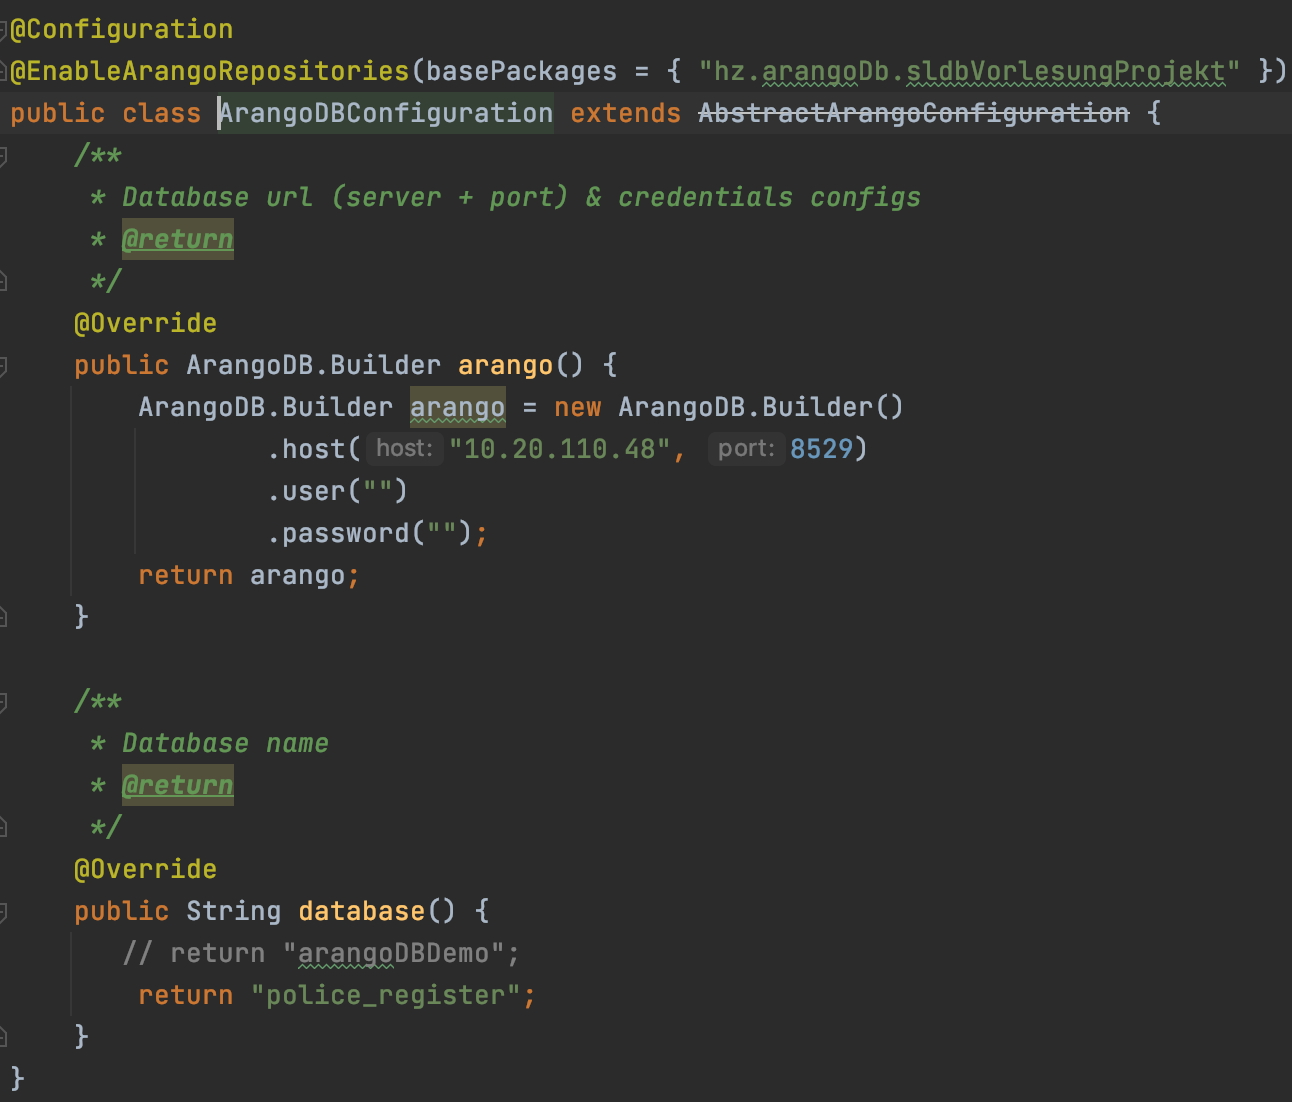
\includegraphics[scale=.4]{images/dbConfig}
\captionof{figure}{Datenbank-Konfiguration}
\end{center}

.\subsubsection{Schnittstelle nach Außen}
SpringBoot bietet auch die Möglichkeit, eine REST-API zu implementieren und diese über verschiedene HTTP-Methoden verfügbar zu machen. Um einen Controller auf SpringBoot als REST-Schnittstelle zu definieren, fügen Sie einfach die Annotation @RestController hinzu. Danach wird  in jeder Methode des Controllers auch die Annotation @GetMapping , @PostMapping verwenden, um zu definieren, über welche HTTP-Methode diese Ressource exponiert wird.
\subsubsection{Anwendungsszenario 1}

für Anwendungsszenario 1 wurde eine annotierte @RestController-Klasse erstellt, die eine Methode namens GetCarByColor(String carID) enthält. Diese Methode ist ebenfalls mit @GetMapping annotiert, was den Zugriff auf die Ressource über die HTTP-GET-Methode ermöglicht. Diese Methode gibt als Ressource ein Car-Objekt in Form von Json zurück. Um diese Ressourcen zu erhalten, sendet Java eine AQL-Abfrage mit der Car-Color des zu suchenden Autos an die ArangoDB-Datenbank. ArangoDB wiederum sucht das Auto und gibt das Ergebnis des gefundenen Autos zurück. 

\begin{center}
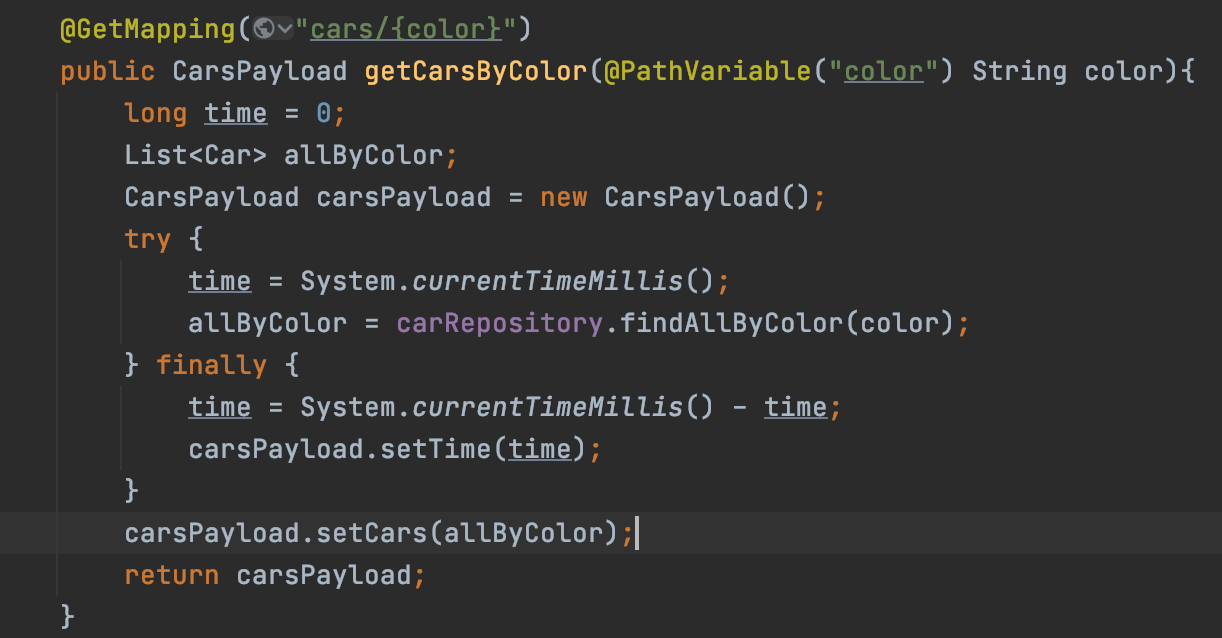
\includegraphics[scale=.4]{images/carByColor}
\captionof{figure}{Code: Auto über Color abfragen}
\end{center}

\subsubsection{Anwendungsszenario 2}
Analog zum vorherigen Anwendungsszenario 1 wurde eine Methode getCarById(String car-Id) mit der Annotation @GetMapping erstellt. Diese Methode sendet eine AQL-Anfrage an die Datenbank und gibt ein Objekt Car zurück.

\begin{center}
\includegraphics[scale=.4]{images/carById}
\captionof{figure}{Code: Auto über ID abfragen}
\end{center}

\subsubsection{Anwendungsszenario 3}

für das dritte Anwendungsszenario geht es darum, eine statistik über die verschiedenen Modelle von Autos zu erstellen, die üblicherweise kollidieren. die Implementierung dieser Methode erfolgt ebenfalls wie oben beschrieben. auch diese Methode wird mit @GetMapping annotiert.

\begin{center}
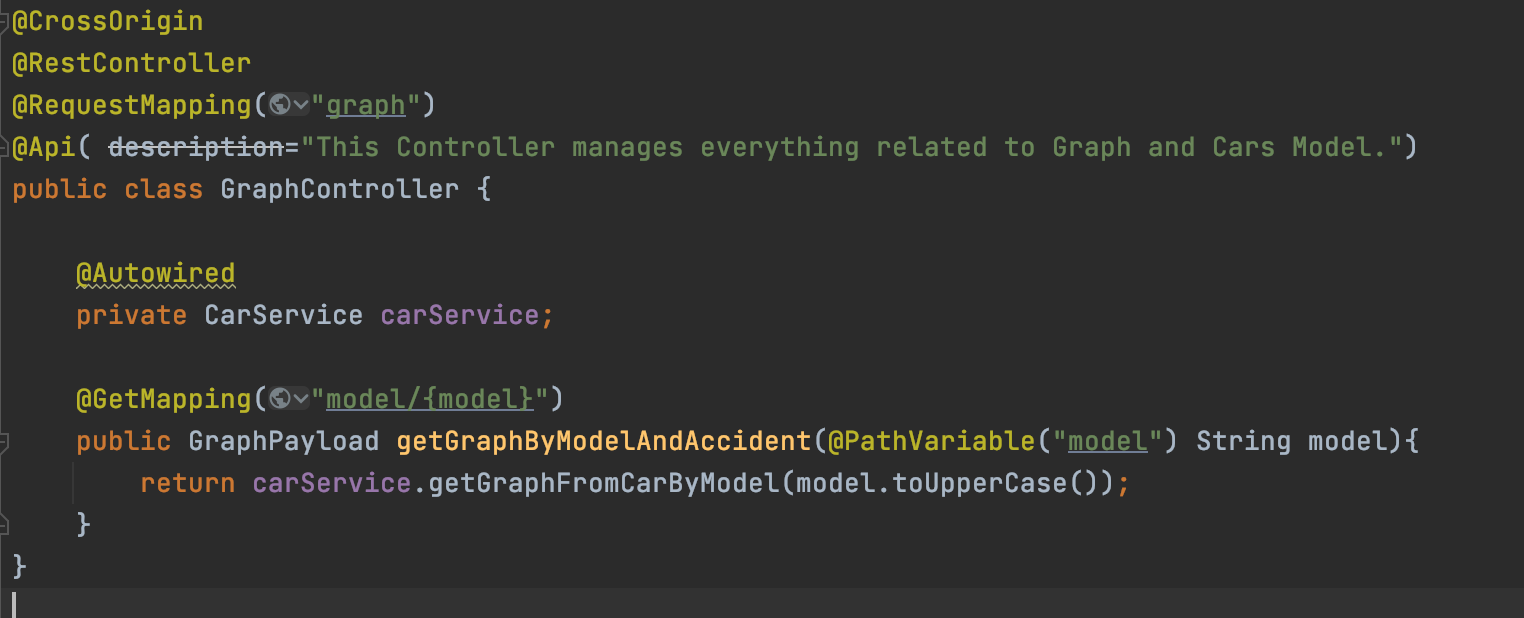
\includegraphics[scale=.4]{images/carModel}
\captionof{figure}{Suche im Graph}
\end{center}